%%%%%%%%%%%%%%%%%%%%%%%%%%%%%%%%%%%
\subsection{Purity Monitors}
\label{sec:fdsp-slow-cryo-purity-mon}
%Laura
A purity monitor (PrM) is a standalone miniature TPC which measures the lifetime of photoelectrons generated by a UV-illuminated gold photocathode in order to measure a given substance's purity. It has high sensitivity to the purity of liquid argon and does not rely on the LArTPC high voltage, electronics, and data acquisition. PrMs are important detectors for guaranteeing successful commissioning and operation of the LArTPC and meet the requirement to measure position-dependent purity necessary to achieve DUNE's physics goal. The purity monitors also have the potential to be developed as a calibration tool that provides high precision and real-time electron lifetime measurements for wire-by-wire detector calibration. 


\subsubsection{Physics and Simulation}
%Andrew will add something here in the next day.


\subsubsection{Design}
%Laura
A purity monitor's basic design is based on those used by the ICARUS and LAPD experiments~\cite{Carugno:1990kd, Adamowski:2014daa} (Figure~\ref{fig:PrMon}). It is a double-gridded ion chamber immersed in the liquid argon volume. It measures the electron drift lifetime between its anode and cathode. The electrons are generated by the purity monitor's UV-illuminated gold photocathode. The UV is generated by a xenon flash lamp. The electron lifetime in liquid argon is inversely proportional to the electronegative impurity concentration. The fraction of electrons generated at the cathode that arrive at the anode ($Q_A/Q_C$) after the electron drift time $t$ is a measure of the electron lifetime $\tau$: $Q_A/Q_C=e^{-t/\tau}$. 

%\begin{dunefigure}[Purity Monitor]{fig:PrMon}
%  {Overall design of the individual purity monitors devices which are immersed into the LAr.}
%  \includegraphics[width=0.3\textwidth]{PrMon.pdf}%
%\end{dunefigure}


\subsubsection{Production and Assembly}
\label{sec:PrMon-Production-Assembly}
%Andrew
Production of the individual purity monitors and the assembly of them into the string that will be placed into the DUNE-FD cryostat will follow the same methodology that is being developed for ProtoDUNE.  Each of the individual monitors will be fabricated, assembled and then tested in a smaller test stand.  After confirming that each of the individual purity monitors operates at the required performance, they would be assembled together via the support tubes used to mount the system to the inside of the cryostat such that three purity monitors are grouped together to form a "string" of purity monitors, as shown in Fig.~\ref{fig:PrMon-SystemString}.  The assembly of the individual purity monitors into the string would follow the steps laid out in Fig.~\ref{fig:PrMon-StringAssembly}.  

%\begin{dunefigure}[Purity Monitor String]{fig:PrMon-SystemString}
%  {Design of the purity monitor string that will contain three purity monitors.}
%  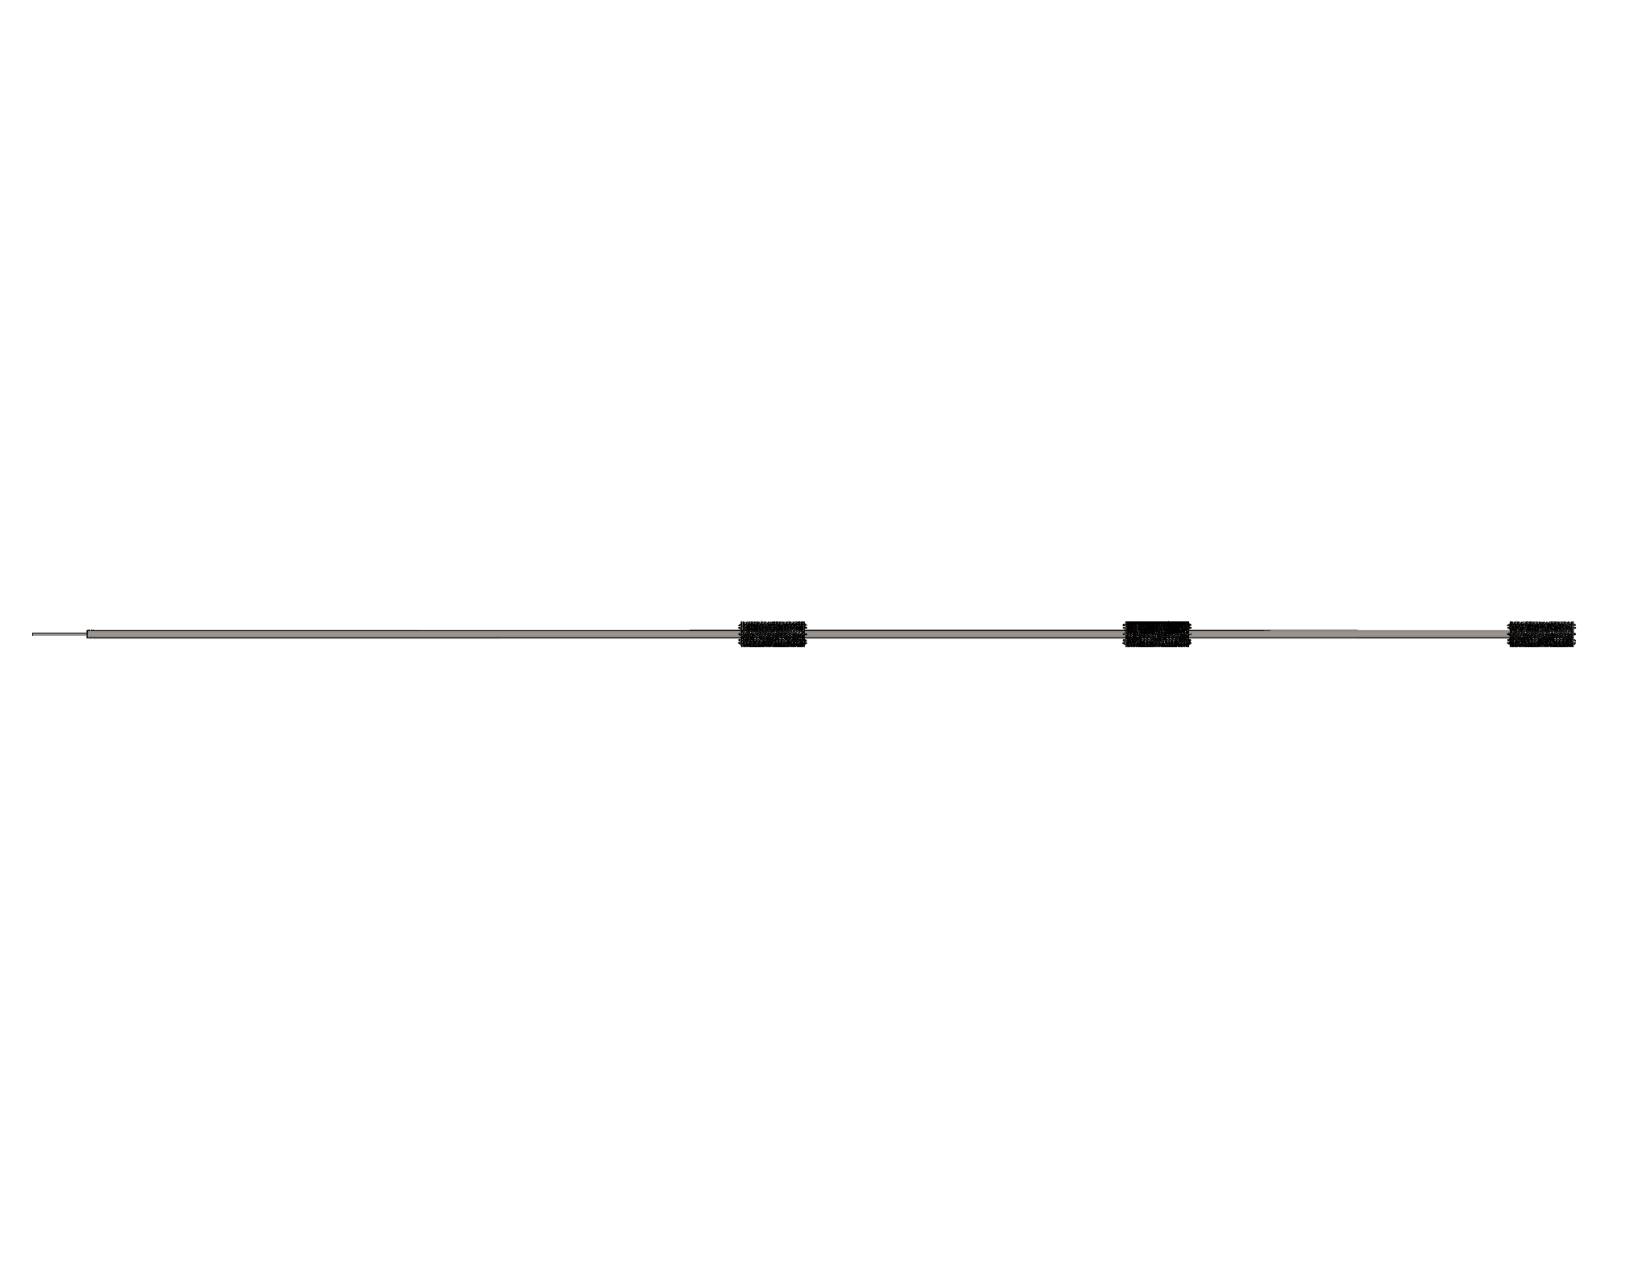
\includegraphics[width=0.3\textwidth]{PrMon-SystemString.pdf}%
%\end{dunefigure}

%\begin{dunefigure}[Purity Monitor String Assembly]{fig:PrMon-SystemString}
%  {Assembly sequence of the purity monitor string.}
%  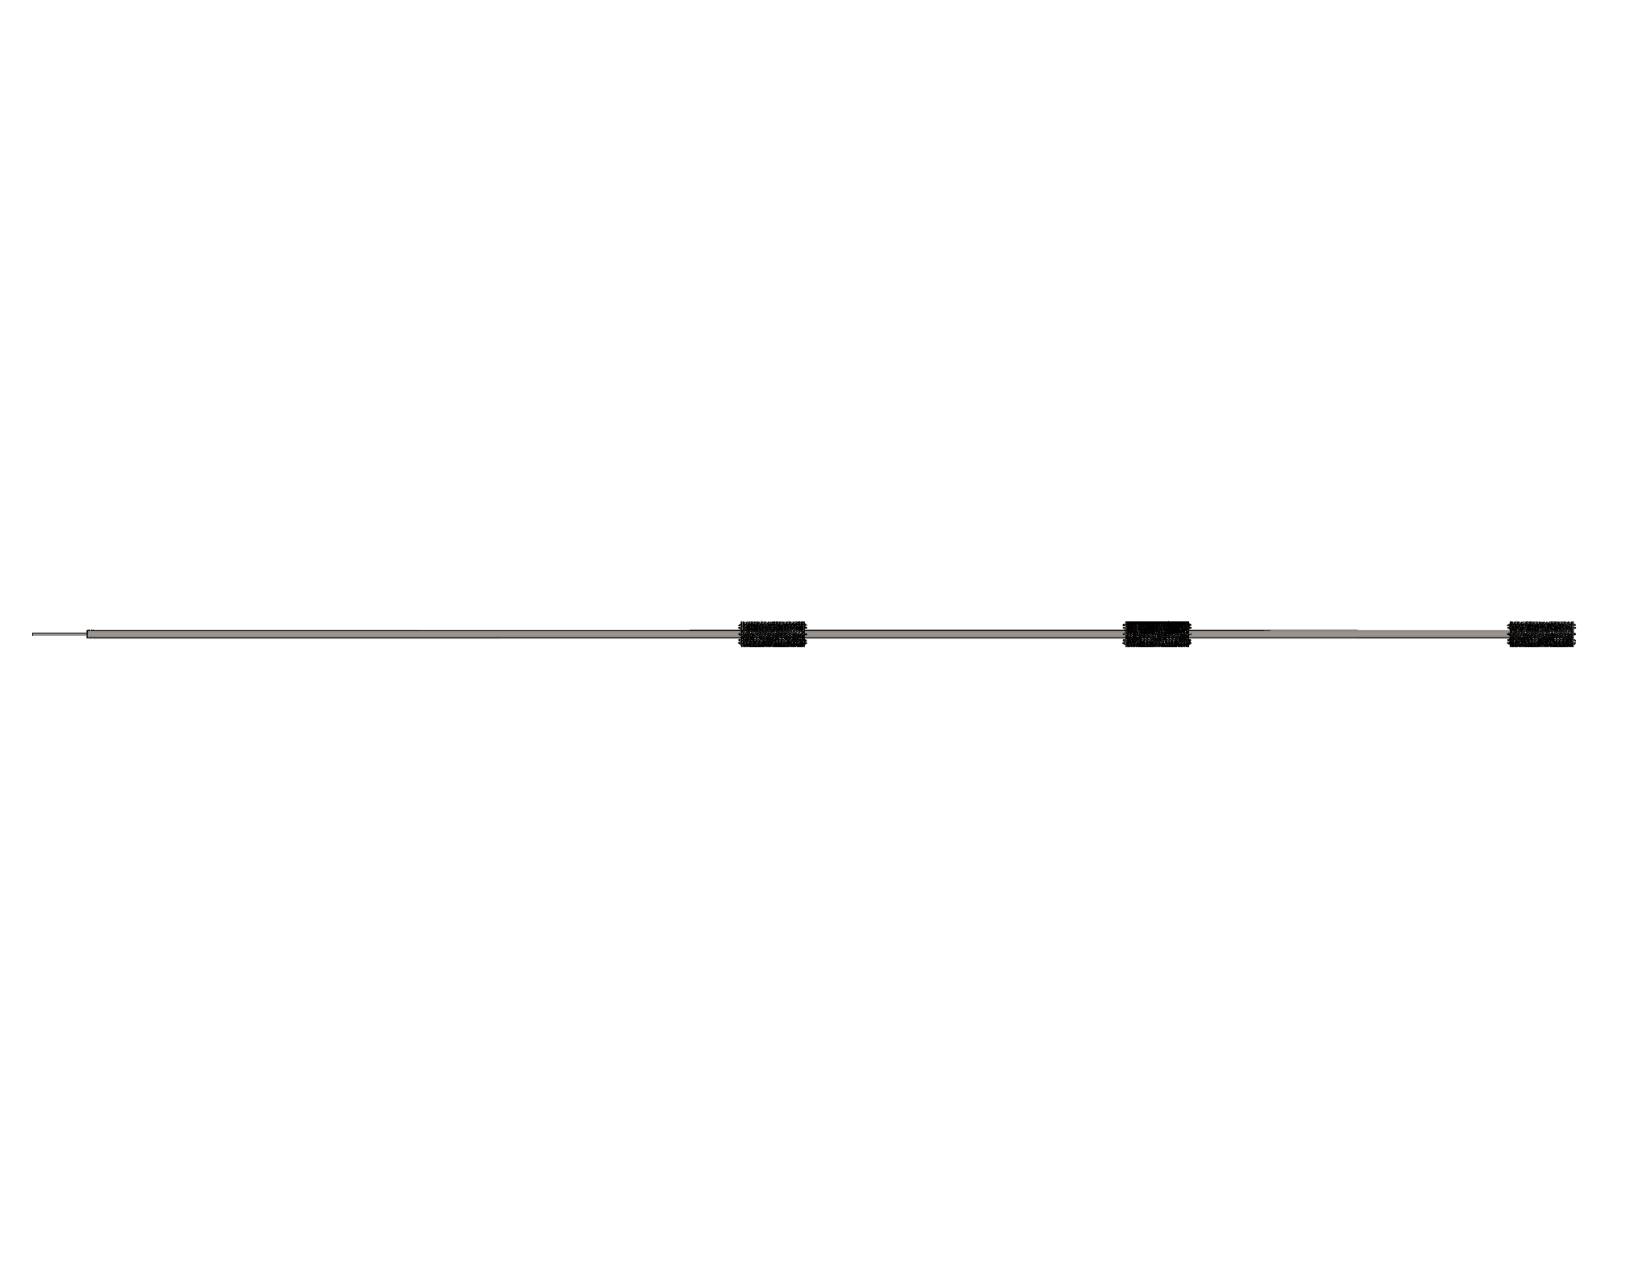
\includegraphics[width=0.3\textwidth]{PrMon-SystemString.pdf}%
%\end{dunefigure}


\subsubsection{Slow Controls Interfacing}
%Jianming


\subsubsection{Installation, Integration and Commissioning}
\label{sec:PrMon-Install-Integrate-Commission}
%Andrew
The purity monitor system will be built in a modular way, such that is can be assembled outside of DUNE-FD cryostat.  The assembly of the purity monitors themselves would occur outside of the cryostat and would include everything described in Sec.~\ref{sec:PrMon-Production-Assembly}.  The installation of the purity monitor system can then be carried out with the least number of steps inside the cryostat.  The assembly itself would come into the cryostat with the three individual purity monitors mounted to the support tubes and no HV cables or optical fibers installed yet.  The support tube at the top and bottom of the assembly would then be mounted to the brackets inside the cryostat that could be attached to the cables trays and/or the detector support structure.  In parallel to this work, the front-end electronics and light source can be installed on the top of the cryostat, along with the installation of the electronics and power supplies into the electronics rack.  

Integration would begin by running the HV cables and optical fibers to the purity monitors, coming from the top of the cryostat.  The HV cables would be attached to the HV feedthroughs with enough length to reach each of the respective purity monitors.  The cables would be run through the port reserved for the purity monitor system, along cable trays inside the cryostat until they reach the purity monitor system, and would then be terminated through the support tube down to each of the purity monitors.  Each purity monitor will have three HV cables that connect it to the feedthrough, and then along to the front-end electronics.  The optical fibers would then be run through the special optical fiber feedthrough, into the cryostat, and would be guided to the purity monitor system either using the cables trays or guide tubes.  Which ever solution is adopted for running the optical fibers from the feedthrough to the purity monitor system, it should protect the fibers from accidental breakage during the remainder of the detector and instrumentation installation process.  The optical fibers would then be run inside of the purity monitor support tube and to the respective purity monitors terminating them at the photocathode of each, protecting them from breakage near the purity monitor system itself.

Integration would continue with the connection of the HV cables between the feedthrough and the system front-end electronics, and then optical fibers to the light source.  The cables connecting the front-end electronics and the light source to the electronics rack would also be run and connected at this point.  This would allow for the system to be turned on and the software to begin testing the various components and connections.  Once it was confirmed that all connections had been successfully made, the integration to the slow controls system would be made, first by establishing communications between the two systems and then transferring mach data between them to ensure successful exchange of important system parameters and measurements.  

Commissioning of the purity monitor system would officially be done once the cryostat had been purged and a gaseous argon atmosphere was present.  At this point the HV for the purity monitors could be ramped up without the fear of discharge through the air, and the light source the turned on.  Although the drift electron lifetime in the gaseous argon would be very large and therefore not really measurable with the purity monitors themselves, the signal strength at both the cathode and anode would give a good indication of how well the light source is generating drift electrons from the photocathode and that they are successfully drifted to the anode by looking at the signal strength at the anode and comparing it to that of the cathode.


%\subsubsection{Quality Control}
%This subsubsection has been moved to the official Quality Control subsection and the text has already been provided by Andrew, please double check it and confirm that is it fine and feel free to recommend suggestions for improvement.